\graphicspath{{figures_supplement/}}          % graphics
\renewcommand{\thefigure}{S\arabic{figure}}
\renewcommand{\thetable}{S\arabic{table}}

\clearpage
\setcounter{page}{1}
\setcounter{section}{1}
\setcounter{figure}{0}

\section*{Supplement}

\begin{figure*}[th]
  \includegraphics[width=12cm]{ozone_timeseries_fennoscandic_obs.png}
  \caption{Time series of ozone observations in northern Fennoscandia (Tab.~\ref{tab:ebas_obs}) (1986--2019). Data from EBAS until December 2018. The hatched areas indicate periods with insufficient quality control according to \citet{NILU2003}. (a) Esrange (SWE); (b) Janiskoski (RUS); (c) Jergul/Karasjok (NOR); (d) Pallas (FIN); (e) Svanvik (NOR).}
  \label{fig:ozone_timesseries_fenoscandic_obs}
\end{figure*}

\begin{figure*}[th]
  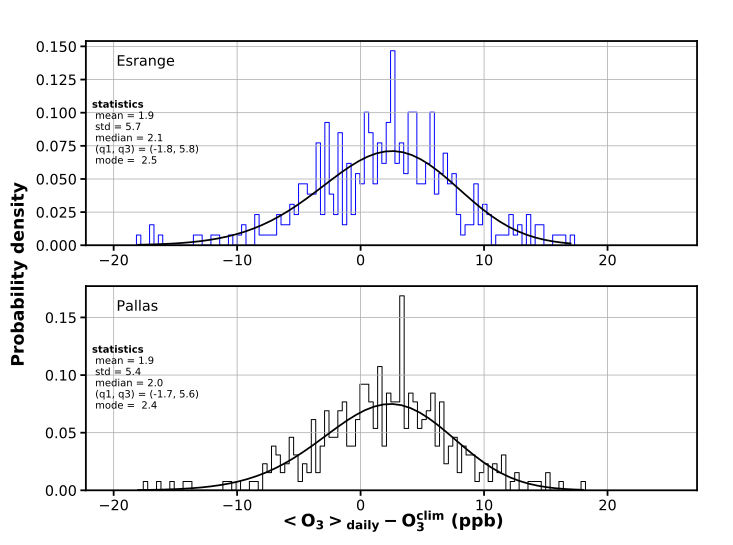
\includegraphics[width=12cm]{ozone_climatology_fenoscandic_obs_residuals}
  \caption{Probability density functions of ozone concentration residuals. 2018 with respect to respective climatology for different sites in Fennoscandia. (a) Esrange; (b) Pallas.}
  \label{fig:ozone_climatology_fenoscandic_obs_residuals}
\end{figure*}

\begin{figure*}[th]
  \includegraphics[width=12cm]{ozone_climatology_fenoscandic_obs_residuals-Svanvik}
  \caption{Probability density functions of ozone concentration residuals. 2018/19 observations at Svanhovd with respect to derived climatologies for (a) Northern Fennoscandia; (b) Svanvik.}
  \label{fig:ozone_climatology_fenoscandic_obs_residuals-Svanvik}
\end{figure*}

\begin{figure*}[th]
  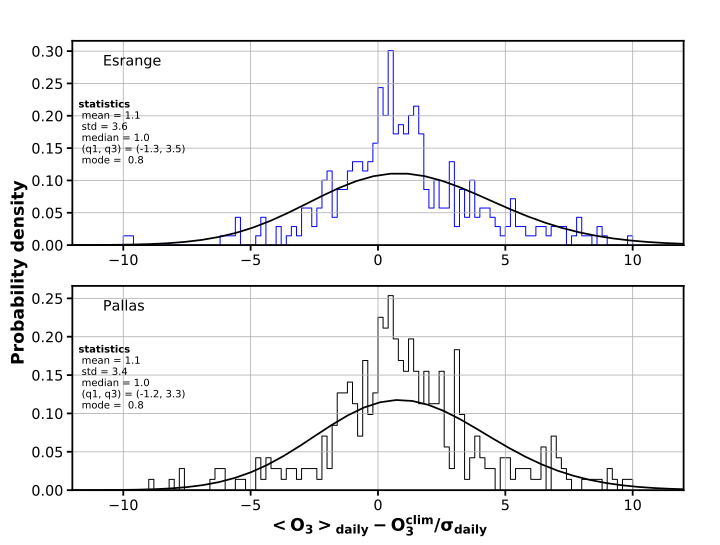
\includegraphics[width=12cm]{ozone_climatology_fenoscandic_obs_test}
  \caption{Student's t-test assuming same sample uncertainty in both, climatology and 2018 observations for different sites in Fennoscandia. \chem{\Delta[O_3]} in Fig.~\ref{fig:ozone_climatology_fenoscandic_obs_residuals} are significantly different from zero-hypothesis on the $1\,\sigma$ level. (a) Esrange; (b) Pallas.}
  \label{fig:ozone_climatology_fenoscandic_obs_test}
\end{figure*}

\begin{figure*}[th]
  \includegraphics[width=12cm]{ozone_climatology_fenoscandic_obs_test-Svanvik}
  \caption{Student's t-test assuming same sample uncertainty in both, climatology and 2018/19 observations at Svanhovd with respect to derived climatologies for (a) Northern Fennoscandia; (b) Svanvik. \chem{\Delta[O_3]} in Fig.~\ref{fig:ozone_climatology_fenoscandic_obs_residuals}a) are significantly different from zero-hypothesis on the $2\,\sigma$,  $1\,\sigma$ level, respectively. \chem{\Delta[O_3]} in Fig.~\ref{fig:ozone_climatology_fenoscandic_obs_residuals}b) are not significantly different from zero-hypothesis.}
  \label{fig:ozone_climatology_fenoscandic_obs_test-Svanvik}
\end{figure*}

\begin{figure*}[th]
  \centering
  \includegraphics[width=1\textwidth]{supplements/supplement_do3se-parameterization_v2}
  \label{tab:do3se_mm_param}
\end{figure*}

\begin{figure*}[t]
  \includegraphics[width=12cm]{greening_season_change_Svanvik}
  \caption{Estimated shift and prolongation of growing season at Svanhovd over the past 6 decades based on data from \citet{SeNorge}.}
  \label{fig:greening_season_change_Svanvik}
\end{figure*}


